The original data used in this report was the monthly price of crude oil per barrel from 1979 to 2023. It was from the U.S Energy Information Administration. \cite{EIA_2024} In its original state it was interesting but was such a large amount of data that it was condensed before getting plotted. This was done by first uploading a text file copy of the information to a WSL directory. From there it was read with “open()” and “readlines()” commands. From there, the information on lines could be split and put into two lists, one for years and one for prices. To further analyze the price data, another step had to be taken because its base state it was just regarded as strings by python which cannot be treated as normal numbers.\\
	\newline The price list containing strings was modified with a for loop to change it into a list of floats. This newly modified list was then separated every 12 values to find the yearly price averages. These yearly price averages were put into a new list which was then graphed. \\



\begin{figure}
  \centering
  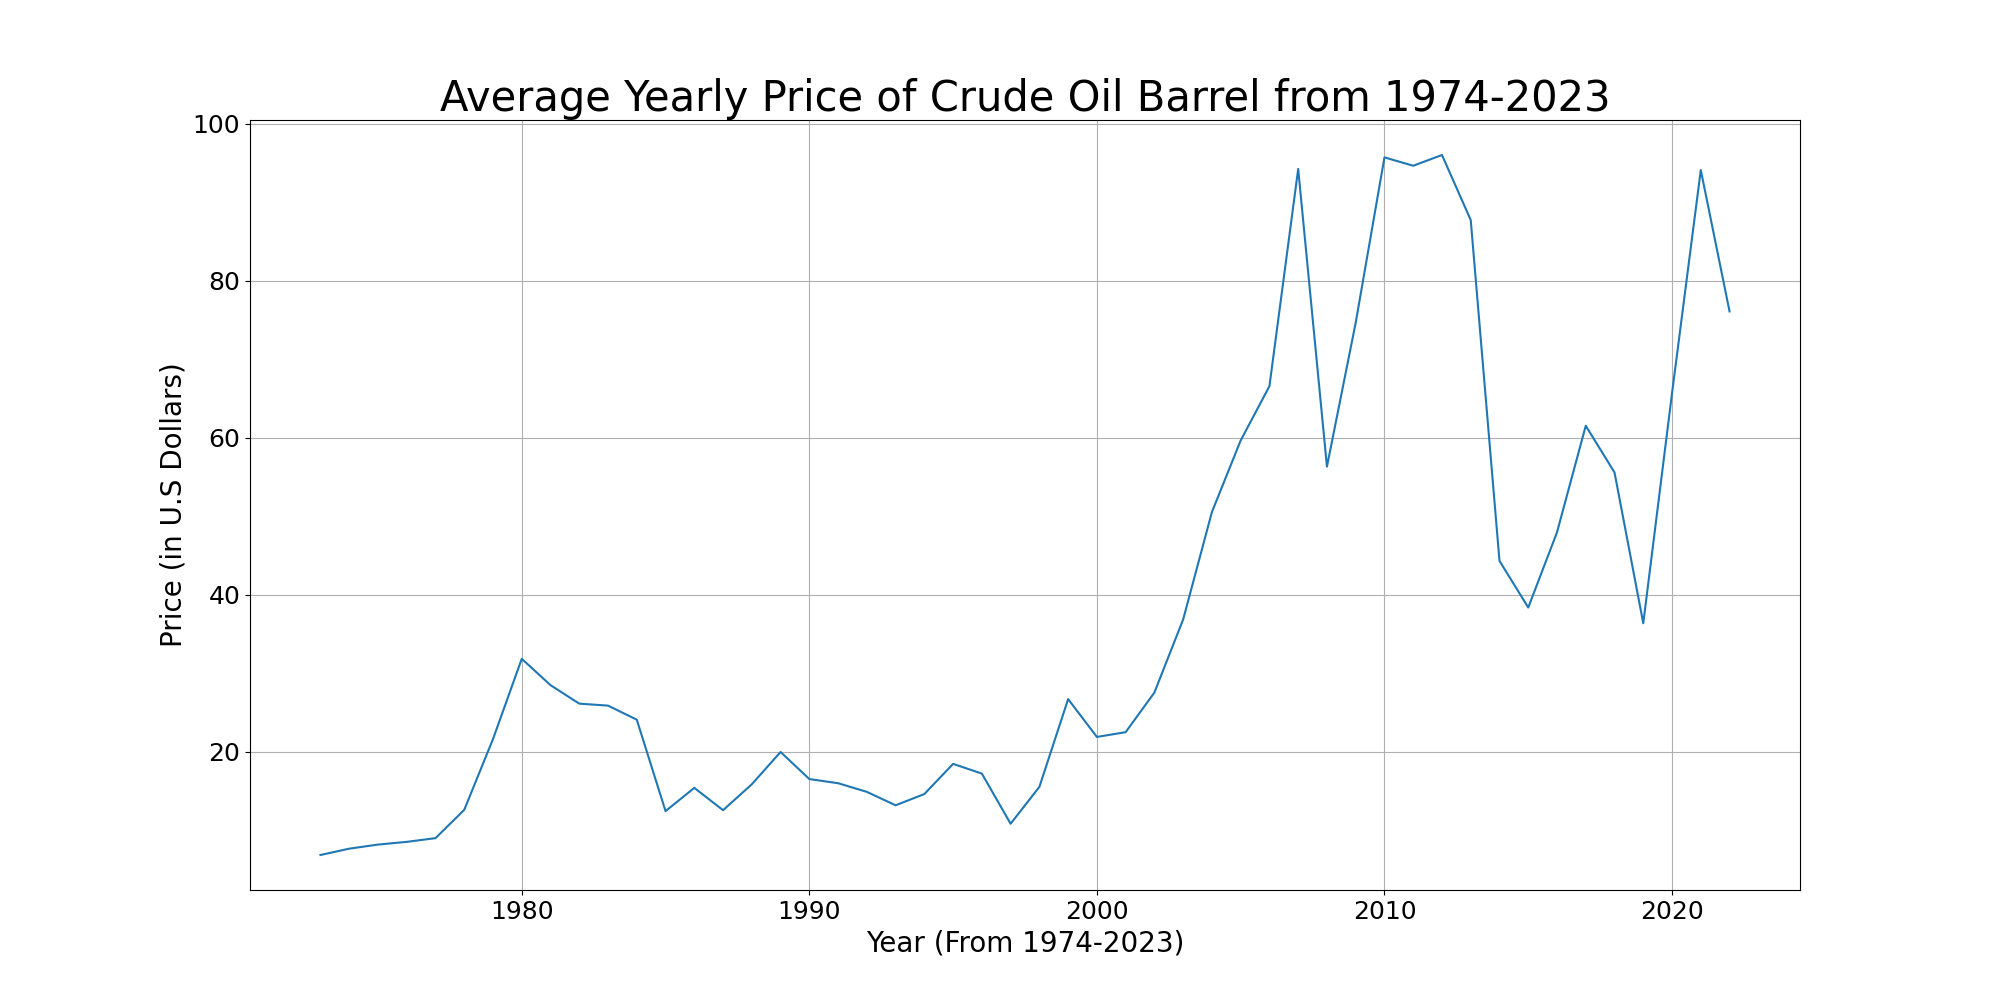
\includegraphics[width=1.0\textwidth]{OilPrice1.png}
  \caption{This is the graph of average Crude oil barrel prices. It was made using the modified lists of data and pylab}
 
  \label{fig:PricePlot}
\end{figure}

 Figure \ref{fig:PricePlot} was made by taking the yearly price averages and putting them in for 
the y values of the plot. The x values were taken from the year list that was made from the original plain text file.
This was done using pylab. Effective Computation in Physics was helpful for doing this. \cite{ECP_2015}
